\documentclass[11pt, a4paper]{article}
%\usepackage{proj1}
\usepackage{natbib}
\usepackage{fancyhdr}  
\usepackage{subcaption}
\usepackage{caption}
\usepackage{graphicx}
\usepackage{numprint}
\usepackage{multirow}
\linespread{1.25} 
\setlength{\parindent}{0cm}
\graphicspath{{Images/}}
\usepackage{hyperref}
\usepackage{amsmath}
\usepackage{amsfonts}
\usepackage{amssymb}
\usepackage{amsthm}
\usepackage{mathtools}
\usepackage{commath}
\usepackage{bbm}

%\usepackage[sc,osf]{mathpazo}
\usepackage{subcaption}
\usepackage[a4paper, top=1in, left=1.0in, right=1.0in, bottom=1in, includehead, includefoot]{geometry} %Usually have top as 1in

\usepackage{listings}
\usepackage{color} %red, green, blue, yellow, cyan, magenta, black, white
\definecolor{mygreen}{RGB}{28,172,0} % color values Red, Green, Blue
\definecolor{mylilas}{RGB}{170,55,241}


\hypersetup{colorlinks,linkcolor={black},citecolor={blue},urlcolor={black}}
\usepackage{color}
\urlstyle{same}


\theoremstyle{definition}
\newtheorem{definition}{Definition}[section]

%\newcommand{\Sta}{\rho}
\newcommand{\adja}{q_a}
\newcommand{\adjb}{q_b}
\newcommand{\adjaB}{q_{a,\partial \Omega}}
\newcommand{\adjbB}{q_{b,\partial \Omega}}
%\newcommand{\Con}{u}
\newcommand{\ra}{\rho_a}
\newcommand{\rb}{\rho_b}
\newcommand{\w}{\mathbf{w}}
\newcommand{\Stav}{\mathbf{v}}
\newcommand{\Adja}{\mathbf{p}}
\newcommand{\Adjb}{q}
\newcommand{\Adjc}{{p}_{\partial \Sigma}}
\newcommand{\Con}{\mathbf{f}}
\newcommand{\n}{\mathbf{n}}
\newcommand{\h}{\mathbf{h}}
\newcommand{\K}{\mathbf{K}}


\pagenumbering{gobble}
\begin{document}

\section*{Flow around a constriction}	
	We are interested in modelling a constriction flow, where the geometry of the channel is set by a steep external potential. This work is loosely replicating the results in the paper by Zimmermann et al. (see Reference).	
	We consider a forward problem of the form:
	\begin{align*}
		\frac{\partial \rho}{\partial t} = D \nabla \cdot \left(\rho \nabla \frac{ \delta \mathcal F}{\delta \rho}\right),
	\end{align*}
	where the free energy includes an ideal gas term, an external potential contribution and an excess free energy functional.
	The excess free energy in the paper is a Ramakrishnan-Yussouff functional, which approximates soft and long-ranged particle interaction and involves the pair direct correlation function. 
	Furthermore, a force term is included, which carries the particles trough the channel along the $x$ axis. This term enters in the external potential contribution to the free energy as $fx$, so that the force in the system is constant with strength $f$. In our framework, this force $f$ is called the flow term.
	The external potential considered in the paper is defined as:
	\begin{align*}
		V_{ext} &= V_0 [1 - 0.5erf((y+g(x))/\sqrt 2 w) + 0.5erf((y-g(x))/\sqrt 2 w)],
	\end{align*}
	where
	\begin{align*}
		g(x) &= L_y /2 - \alpha [1+ \cos(2\pi (x - x_0)/L_c)] \quad \ \text{for} \quad |x - x_0| < L_c/2,\\
		&= L_y /2 \qquad \qquad \qquad \qquad\qquad \qquad \qquad\text{otherwise}\\
		\alpha &= (L_y/4)(1-b),
	\end{align*}
	In the paper the constriction length is $2.686 l$, wall softness is $w = 0.25 l$ and $V_0 = 1000 k_BT$. The choice of channel height is $L_y = \sqrt \frac{\sqrt 3}{2} n l$, with $n = 5$ or $6$  and $L_x = 21.5 l$.  We choose $l = 1$.
	The average density is $\rho_0 = 1/l^2$. Their force is $f = k_bT/l$, which is constant one for us, since we set $k_BT =1$ throughout and $l =1$ as well.
	In the paper a forward problem is run without the force to equilibrate the system and use this as an initial condition for the forced version.
	We use the equilibrium of $\rho$ in absence of particle interactions, which is:
	\begin{align*}
		\rho_0 = e^{-V_{ext}}.
	\end{align*}
\section{Equilibrium}
We choose $N = 50$, $n =30$ and a periodic box from $-3$ to $3$ in both directions. We choose the strength of $V_{ext}$ to be $10$ instead of $1000$ as in the paper. This is to reduce the necessary number of points. If we increase the width of the channel or the strength of the external potential we need considerably more points.
We vary constriction width $b$ and interaction strength $\kappa$ in equilibrium.

For $b = 0.6$ and varying interaction strengths, the results are shown in Figures \ref{F1a}, \ref{F1b} and \ref{F1c}.
\begin{figure}[h]
	\centering
	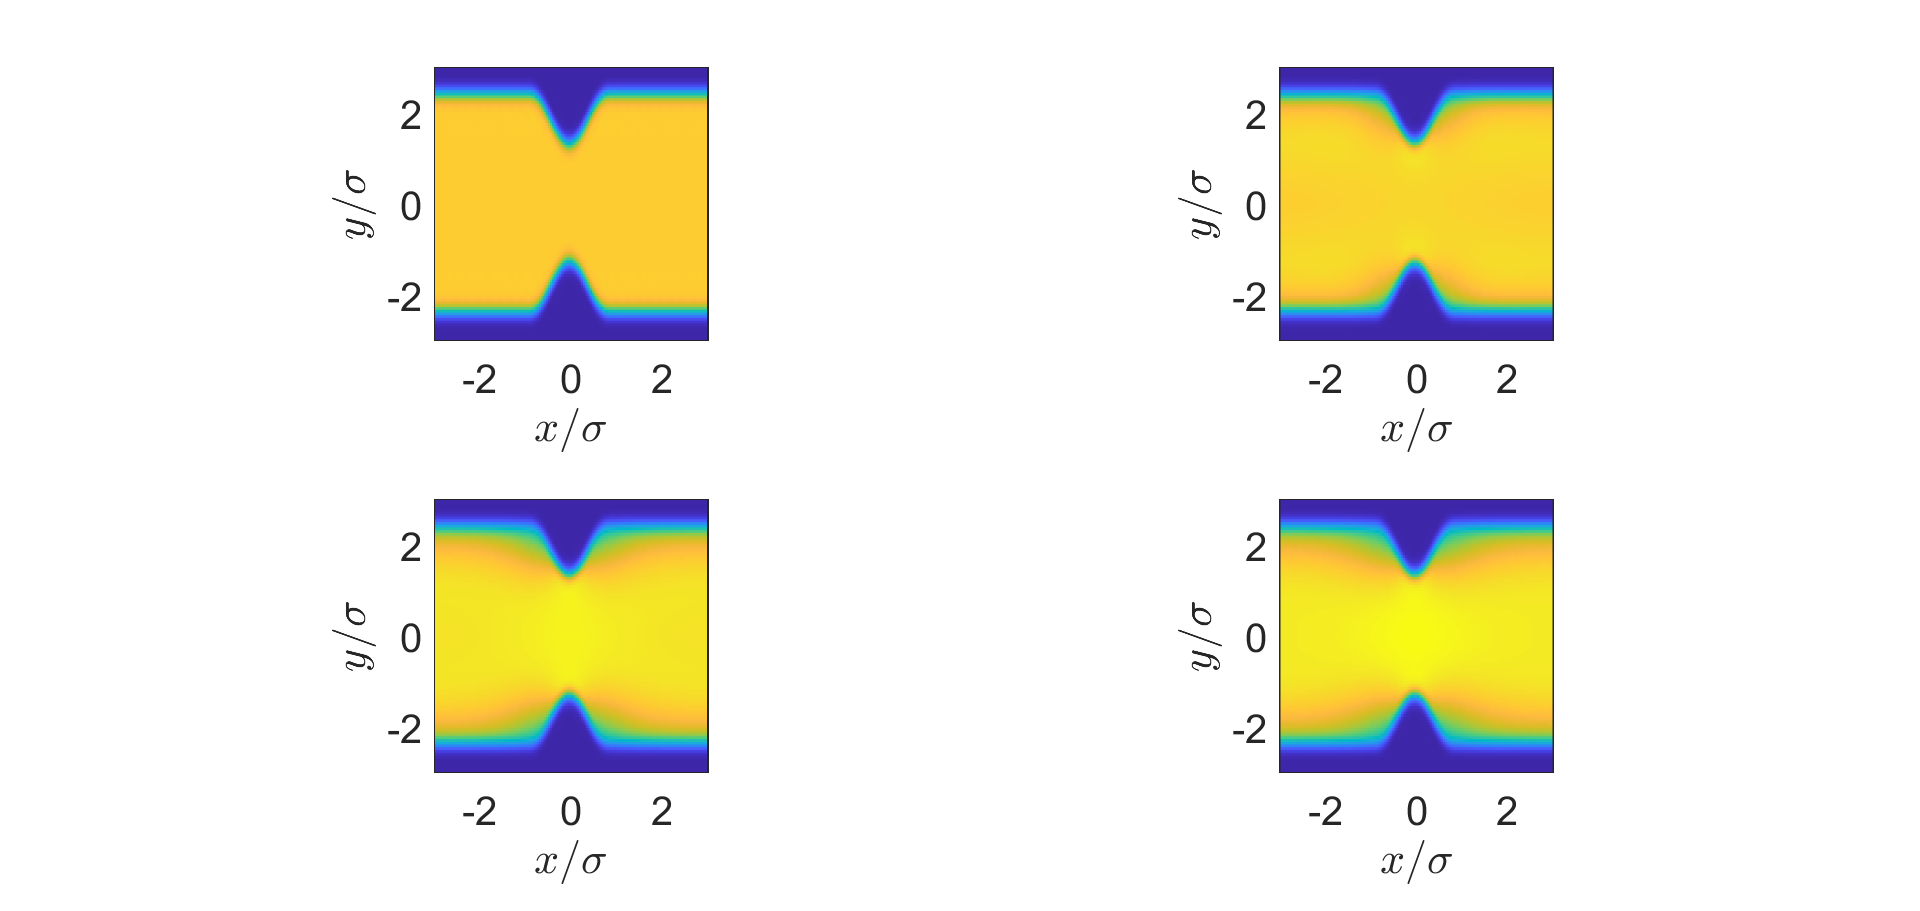
\includegraphics[scale=0.4]{Con1.png}
	\caption{$b = 0.6$, $\kappa =-0.2$} 
	\label{F1a}
\end{figure}

\begin{figure}[h]
	\centering
	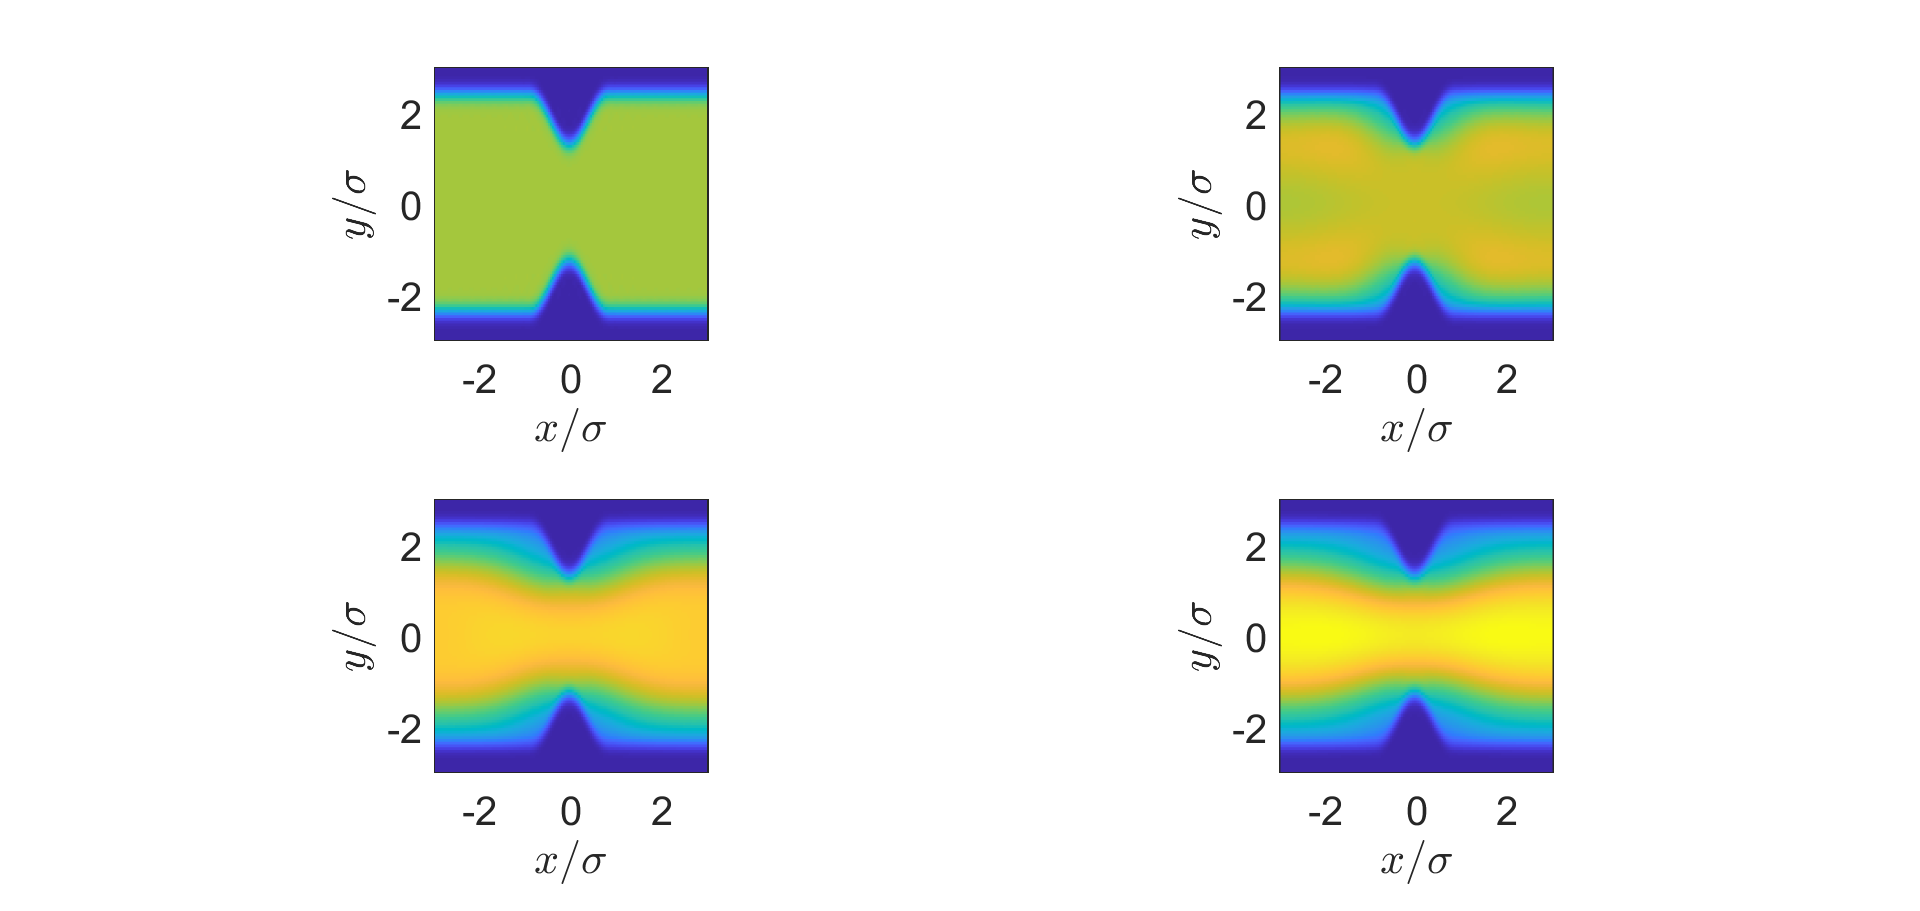
\includegraphics[scale=0.4]{Con2.png}
	\caption{$b = 0.6$, $\kappa =-0.5$} 
	\label{F1b}
\end{figure}
\begin{figure}[h]
	\centering
	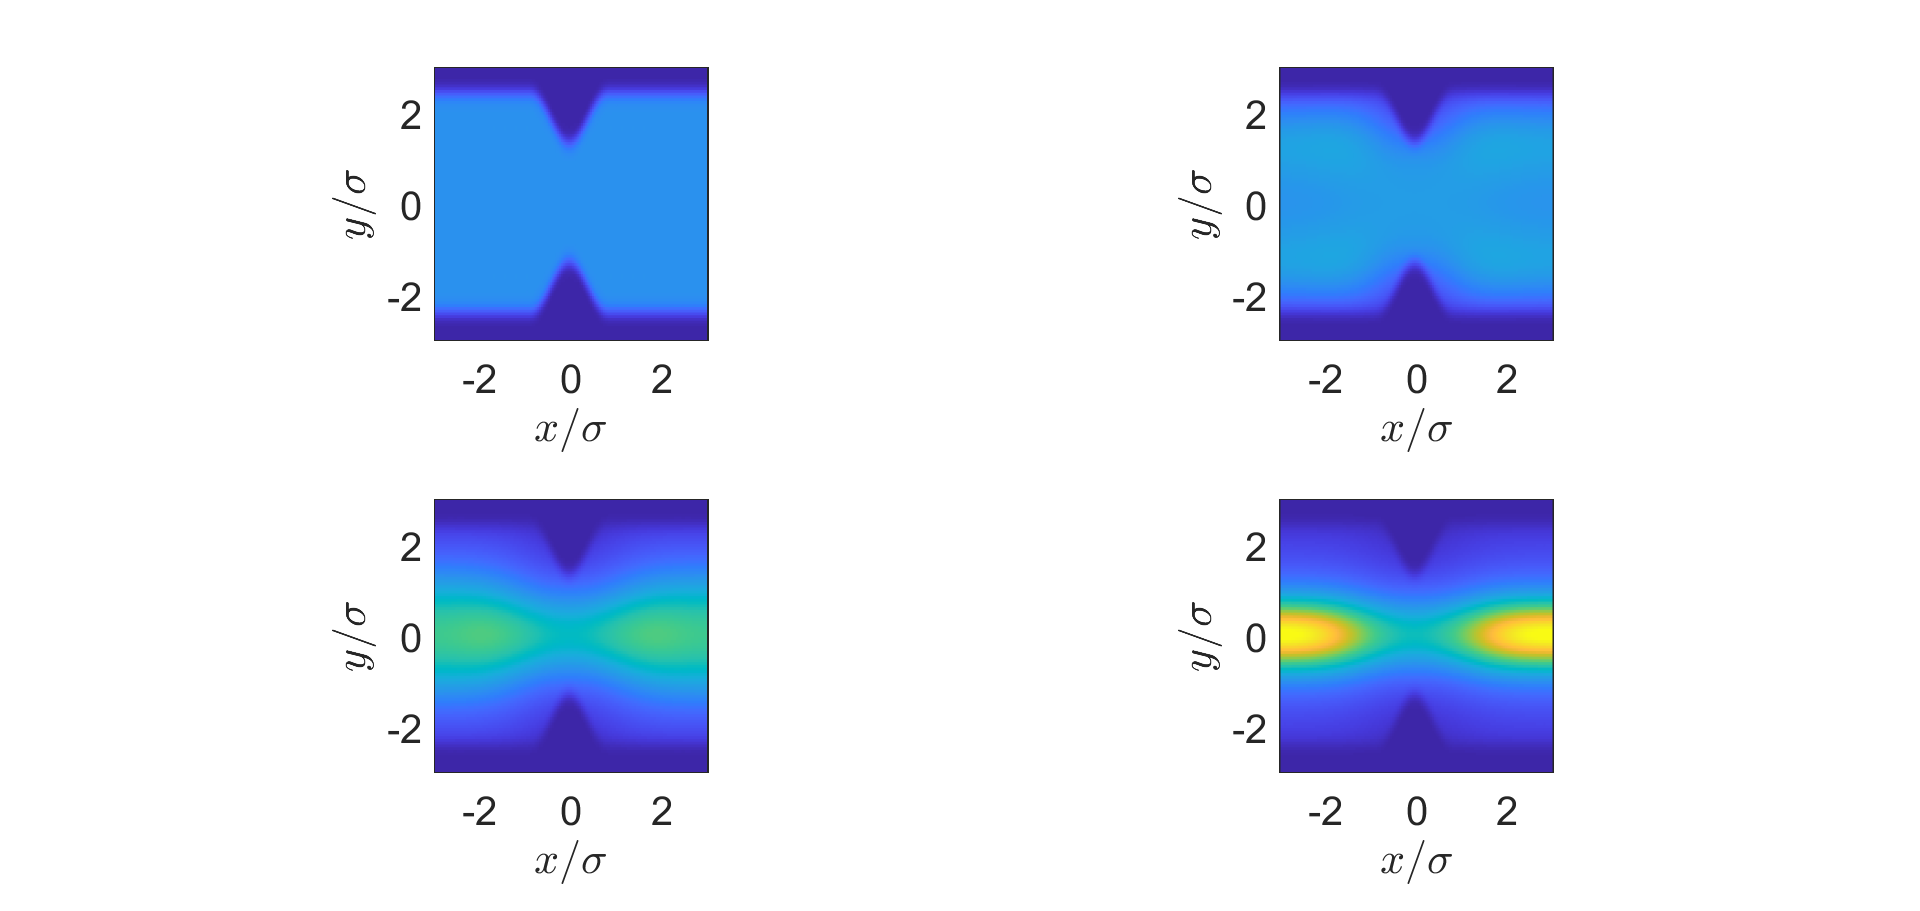
\includegraphics[scale=0.4]{Con3.png}
	\caption{$b = 0.6$, $\kappa =-0.8$} 
	\label{F1c}
\end{figure}
In Figure \ref{F2a} we see how the dynamics changes for a wider constriction $b = 0.8$ as compared to $b = 0.6$ in Figure \ref{F1b}.
\begin{figure}[h]
	\centering
	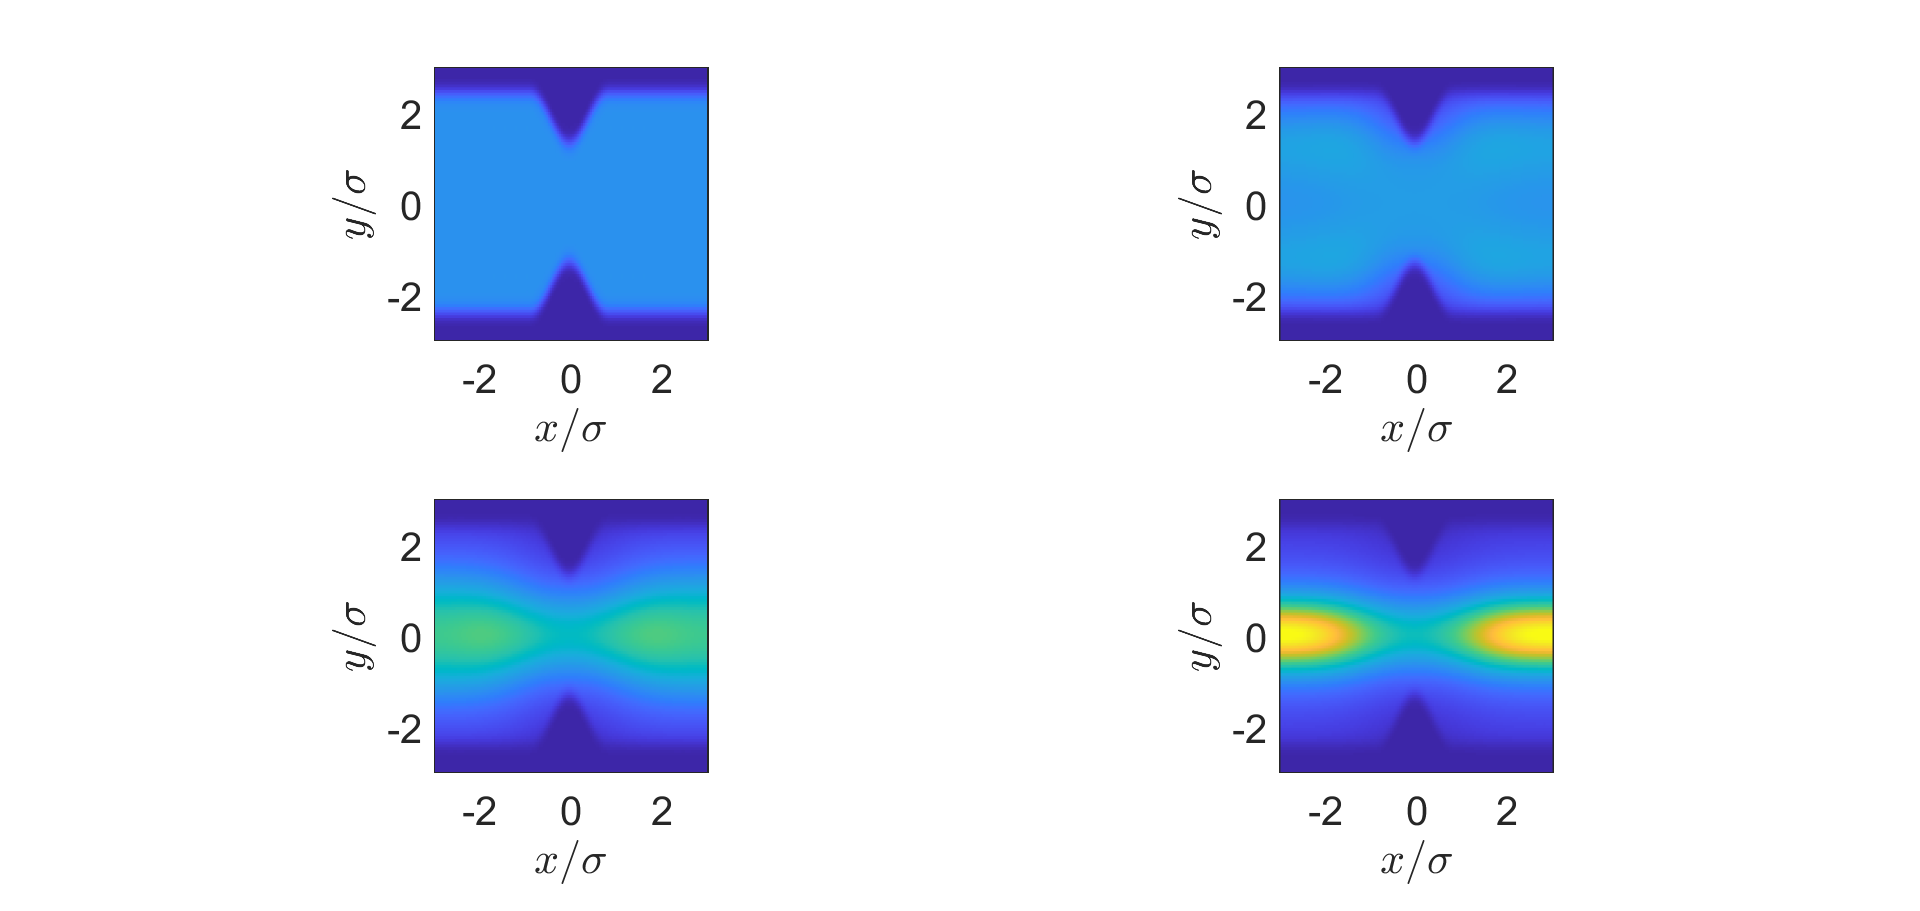
\includegraphics[scale=0.4]{Con3.png}
	\caption{$b = 0.8$, $\kappa =-0.5$} 
	\label{F2a}
\end{figure}

\section{Non-Equilibrium}
We impose a flow of strength one on the equilibrium setup.
For $b = 0.6$ the results are displayed in Figures \ref{F3a}, \ref{F3b}, \ref{F3c} and \ref{F3d}. We can observe that due to the flow particles accumulate at the constriction walls. However, the more attractive the particles are, the more they cluster in the middle of the domain and therefore do not accumulate as much on the constriction walls. 
\begin{figure}[h]
	\centering
	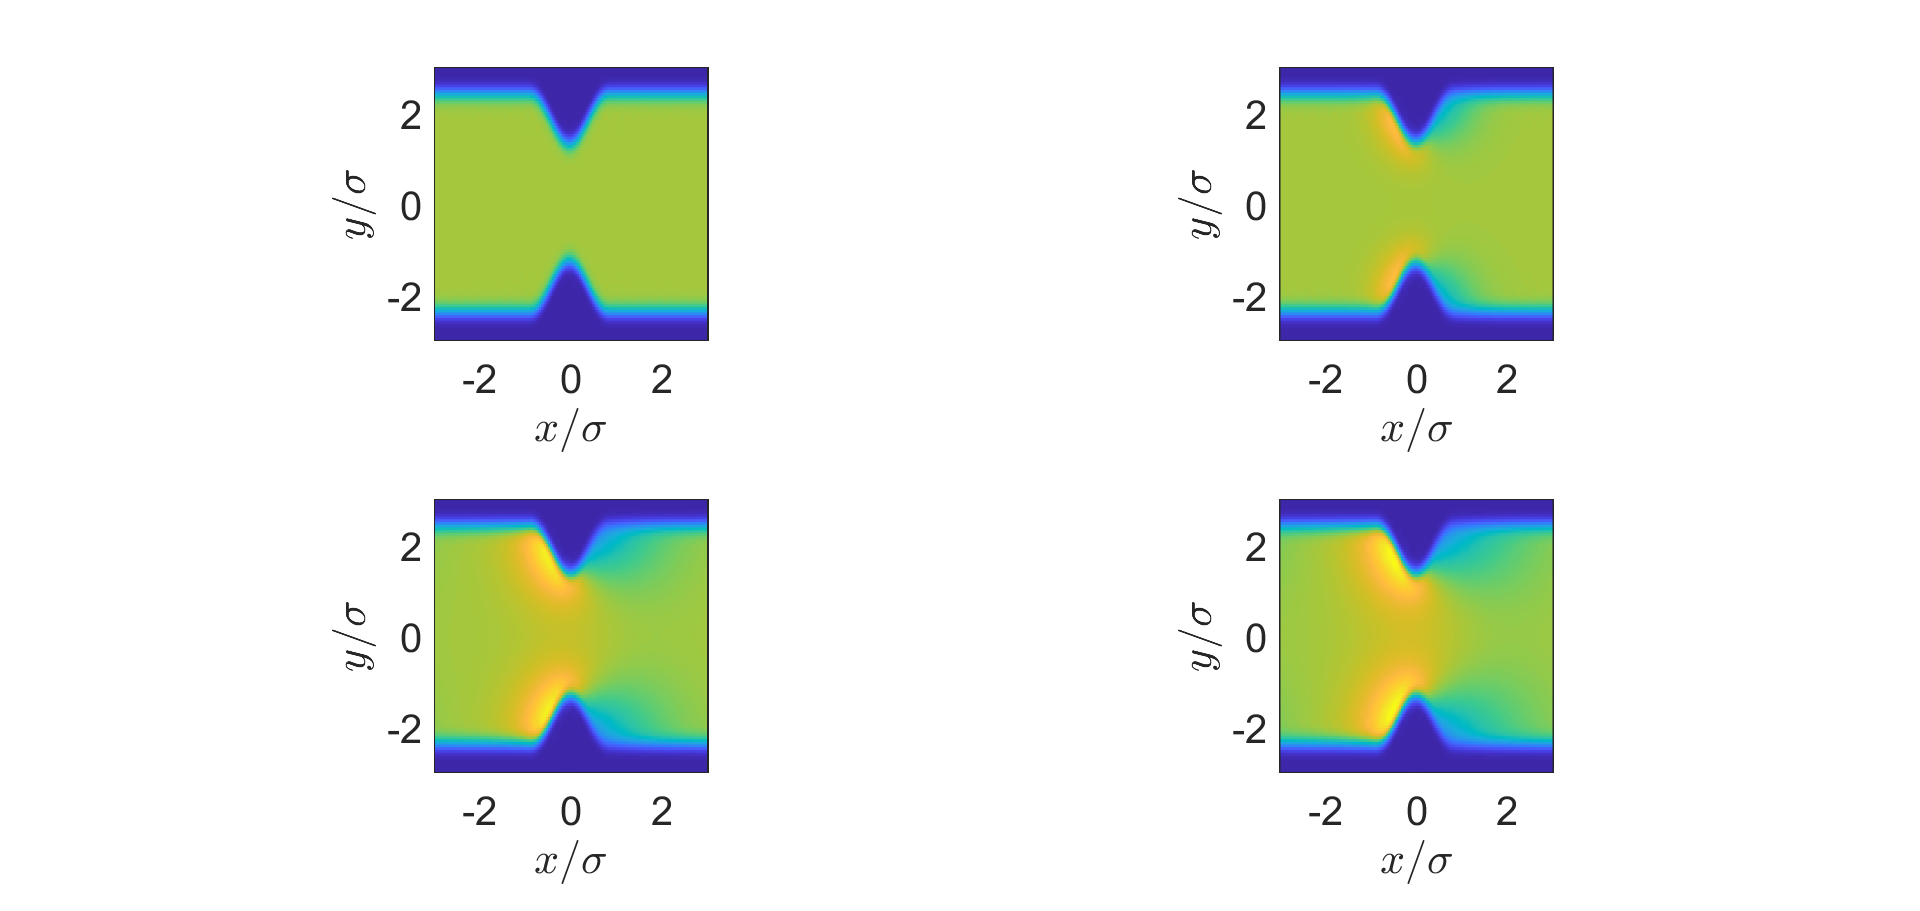
\includegraphics[scale=0.4]{ConFa1.png}
	\caption{$b = 0.6$, $\kappa = 0$} 
	\label{F3a}
\end{figure}

\begin{figure}[h]
	\centering
	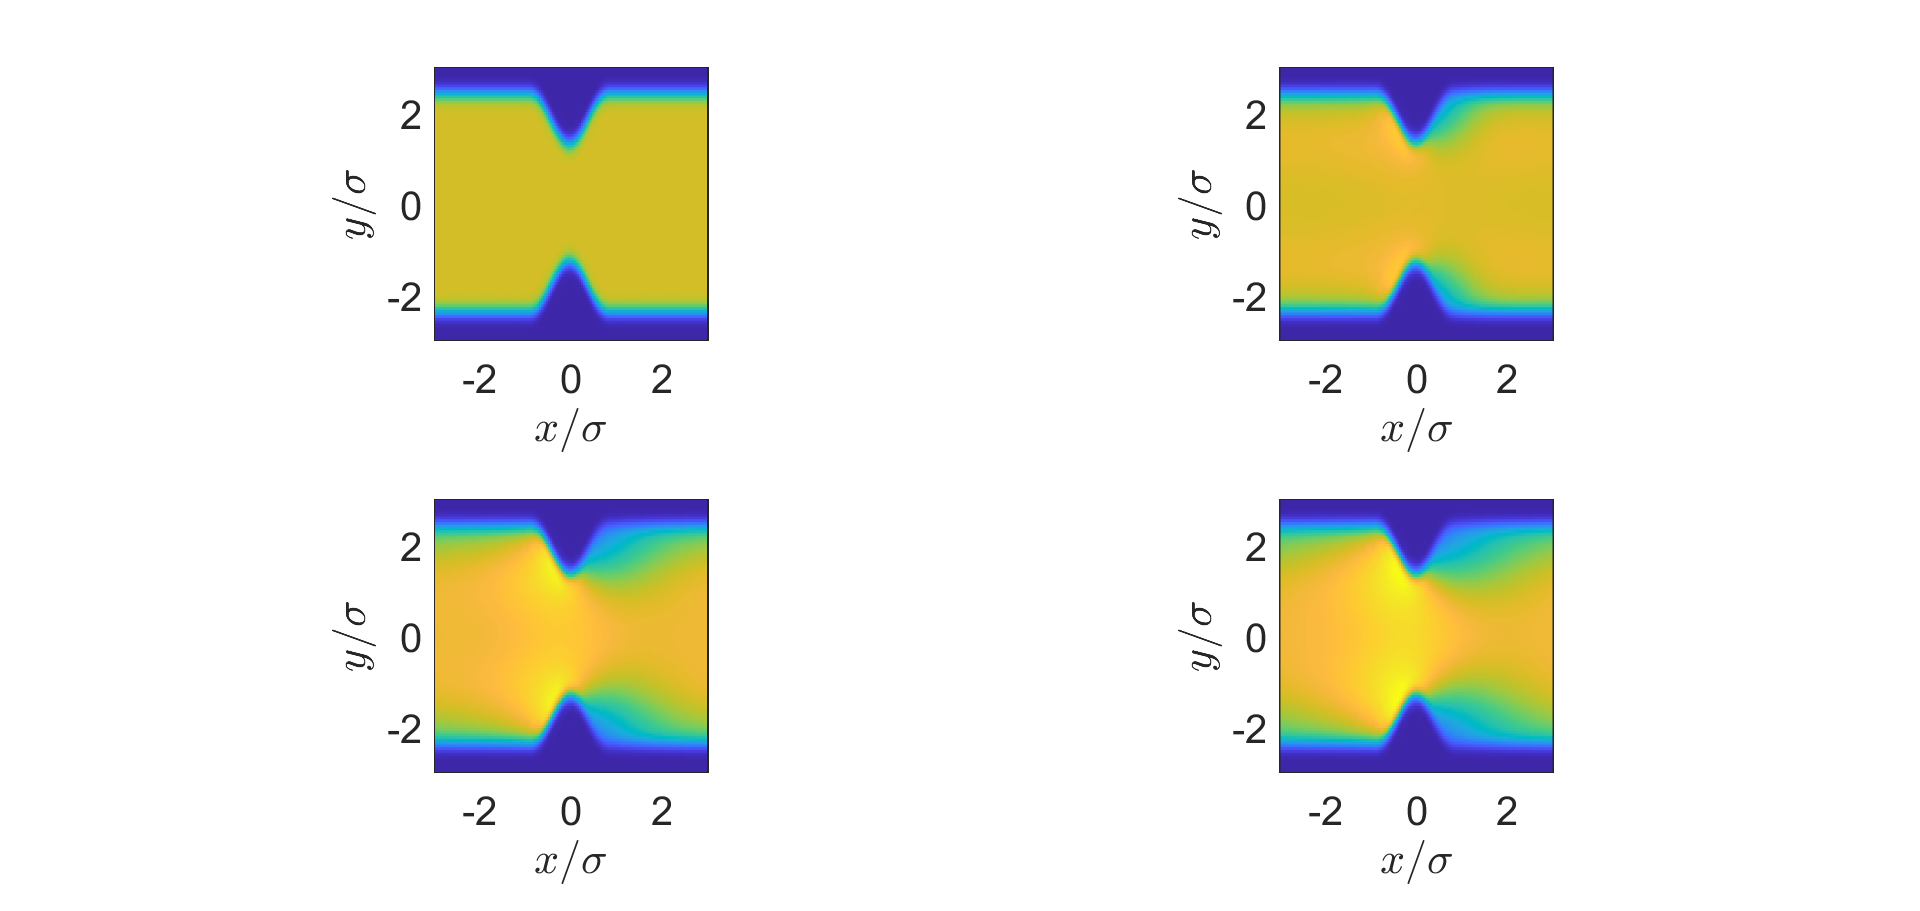
\includegraphics[scale=0.4]{ConFa2.png}
	\caption{$b = 0.6$, $\kappa = -0.2$} 
	\label{F3b}
\end{figure}

\begin{figure}[h]
	\centering
	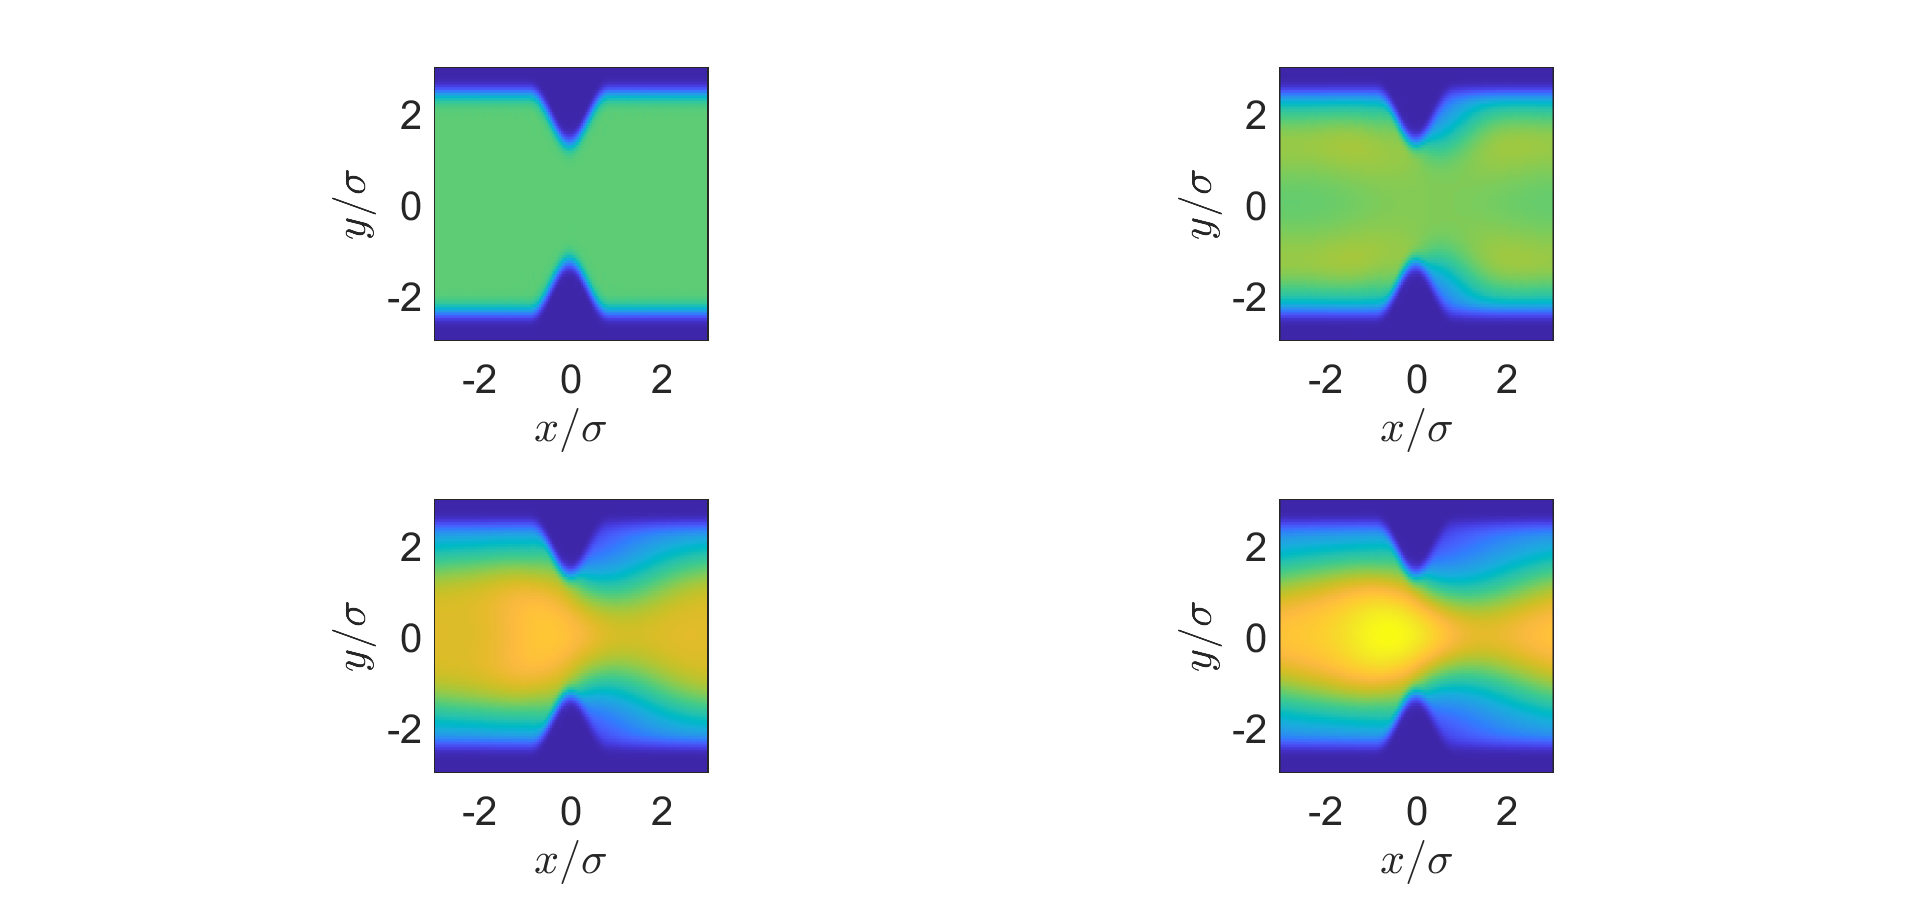
\includegraphics[scale=0.4]{ConFa3.png}
	\caption{$b = 0.6$, $\kappa = -0.5$} 
	\label{F3c}
\end{figure}
\begin{figure}[h]
	\centering
	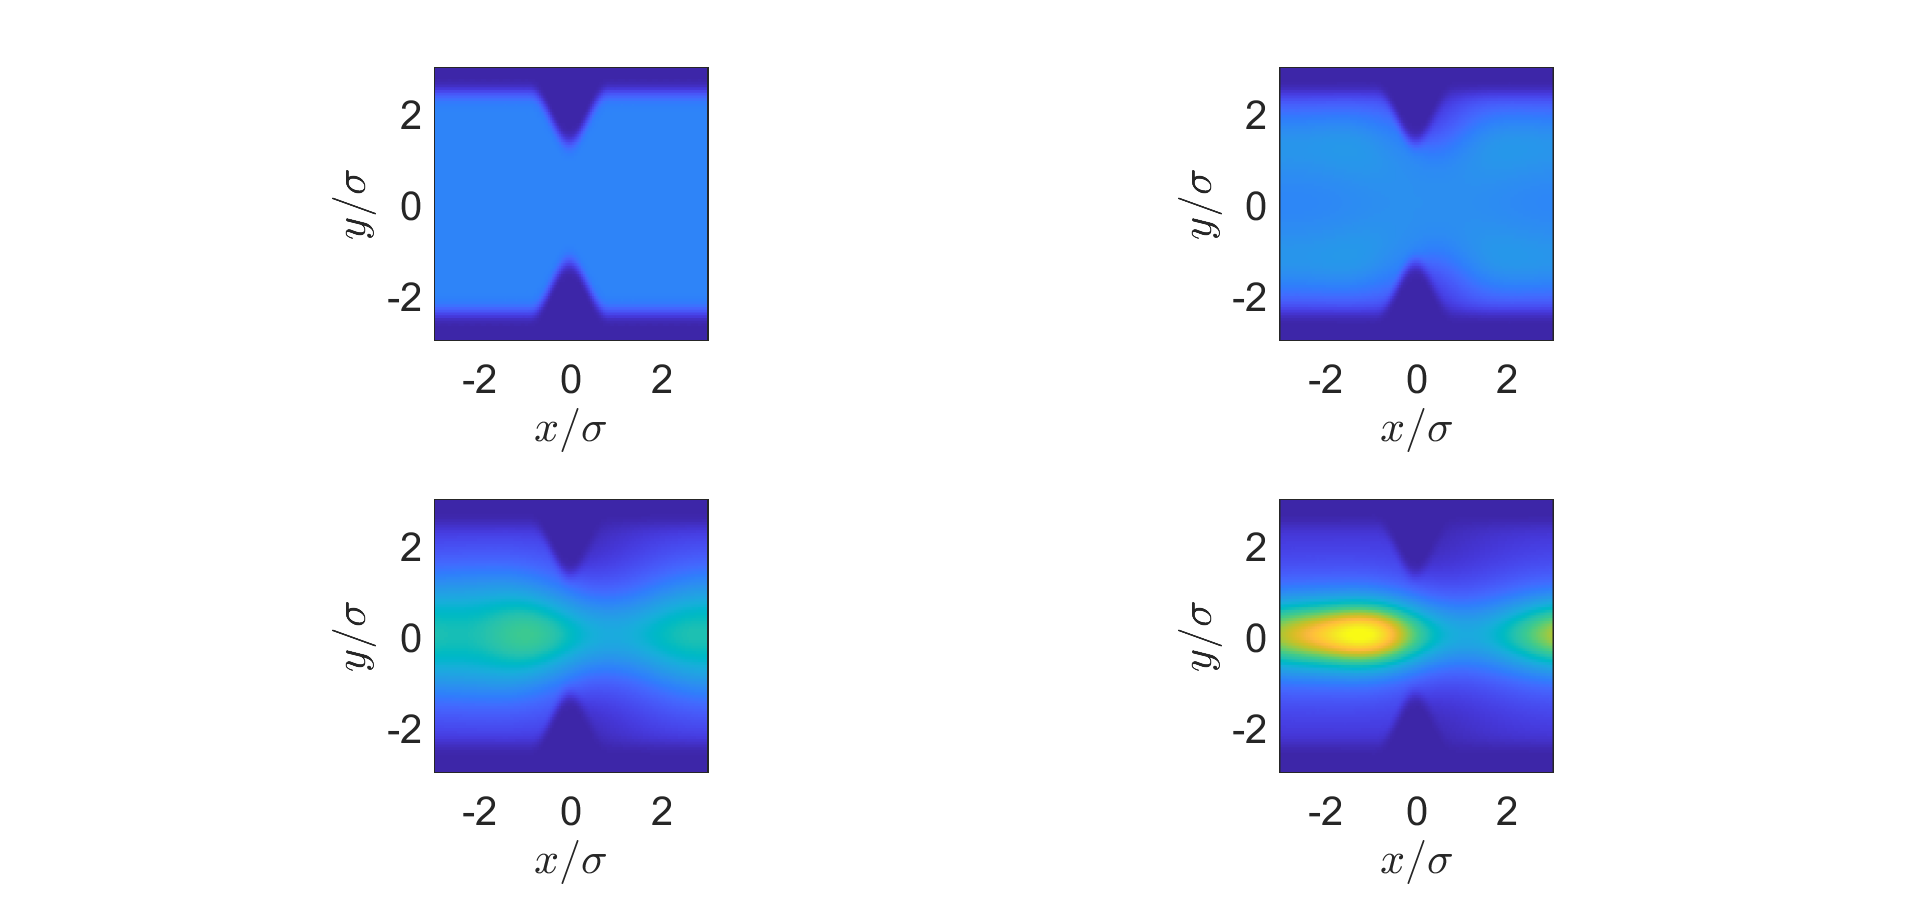
\includegraphics[scale=0.4]{ConFa4.png}
	\caption{$b = 0.6$, $\kappa = -0.8$} 
	\label{F3d}
\end{figure}

\section{Reference}
Zimmermann, Urs \& Smallenburg, Frank \& Löwen, Hartmut. (2015). Flow of colloidal solids and fluids through constrictions: Dynamical density functional theory versus simulation. Journal of Physics: Condensed Matter. 28. 10.1088/0953-8984/28/24/244019. 	
	
\end{document}